Algoritma Genetika (GA) merupakan salah satu metode heuristic yang merupakan cabang dari evolutionary algorithm, yaitu suatu teknik untuk memecahkan masalah-masalah optimasi yang rumit dengan menirukan proses evolusi mahluk hidup. GA terbukti sesuai digunakan untuk menyelesaikan masalah multi objektif. GA berkembang seiring dengan perkembangan teknologi informasi yang sangat pesat \cite{liu2016mining}, \cite{wei2015genetic}.

Algoritma ini banyak digunakan dalam bidang fisika, biologi, ekonomi, sosiologi dan lain-lain yang sering menghadapi masalah optimasi dengan model matematika yang kompleks atau bahkan sulit dibangun \cite{liu2016mining}.

\section{Implementasi Penjadwalan Algoritma Genetika di CodeIgniter}
\par Membuat CRUD dan beberapa table yang akan digunakan seperti pada tahap yang dilakukan sebelumnya, maka untuk mengimplementasikan algoritma genetika yaitu dengan cara melakukan konfigurasi pada model, controller dan views, langkah implementasi algoritma genetika yaitu sebagai berikut:
\begin{enumerate}
    \item Model Algoritma Genetika
    
    \begin{enumerate}
        \item Pada folder \textit{C:/xampp/htdocs/algoritmagenetika/application/models} buat file baru dengan nama \verb|MDL_Jadwal| dan isi codingan seperti berikut:
        
\begin{lstlisting}
<?php
class MDL_Jadwal extends CI_Model{
	function __construct(){
		parent::__construct();
	}
    function get(){
		$rs = $this->db->query(	"SELECT e.nama_hari as hari, 
				Concat_WS('-', concat('(', g.kode_jam), concat( 
			(SELECT kode_jam
				FROM jam
			WHERE kode_jam = 
			(SELECT jm.kode_jam 
				FROM jam jm
			WHERE MID(jm.range_jam,1,5) = MID(g.range_jam,1,5)) + (c.tingkat_kebutuhan - 1)),')')) as sesi,
				Concat_WS('-', MID(g.range_jam,1,5),
			(SELECT MID(range_jam,7,5)
				FROM jam
			WHERE kode_jam = 
			(SELECT jm.kode_jam
				FROM jam jm
			WHERE MID(jm.range_jam,1,5) = MID(g.range_jam,1,5)) + (c.tingkat_kebutuhan - 1))) as jam_kebutuhan,
				c.nama_barang as nama_barang,
				c.tingkat_kebutuhan as tingkat_kebutuhan,
				c.jumlah_dalam_kategori as jumlah_dalam_kategori,
				b.tanggal as tanggal,
				d.nama_vendor as nama_vendor,
				f.nama_bulan_tahun as nama_bulan_tahun
			FROM jadwal a
				LEFT JOIN pengampu b ON a.kode_pengampu = b.kode_pengampu
				LEFT JOIN barang c ON b.kode_barang = c.kode_barang
				LEFT JOIN vendor d ON b.kode_vendor = d.kode_vendor
				LEFT JOIN hari e ON a.kode_hari = e.kode_hari
				LEFT JOIN bulan_tahun f ON a.kode_bulan_tahun = f.kode_bulan_tahun
				LEFT JOIN jam g ON a.kode_jam = g.kode_jam
			Order by e.kode_hari asc,g.kode_jam asc;");
		return $rs;
	}
}
\end{lstlisting}
		\par Keterangan: Fungsinya adalah untuk memanggil semua table yang akan digunakan dalam algortima genetika. Pada codingan tersebut melakukan join terhadap beberapa table yang akan digunakan. Ingat pada saat melakukan join table pastikan table yang dibuat saling berelasi memiliki foreign key dan primary key pada masing-masing table.
    \end{enumerate}
		
    \item Controller Algoritma Genetika
    \begin{enumerate}
	\item Selanjutnya adalah membuat codingan pada folder \textit{C/xampp/htdocs/algoritmagenetika/application/controllers}, buat file dengan nama genetik.php. Pada file genetik.php tersebut didalamnya akan ada function seperti function ambildata, function inisialisasi, function cekfitness, function hitungfitness, function seleksi, function startcrossover, function mutase, dan function getindividu. Function tersebut dibuat secara berurut sesuai dengan urutan proses algoritma genetika.
	
	\item Untuk function ambildata dilakukan select data barang, tahun, bulan dan data vendor untuk dijadikan sebuah chromosome dalam bentuk variable
	
	\item Selanjutnya function inisialisasi, function ini dibuat untuk menentukan jam dan hari secara acak dengan menggunakan fungsi for dan if else
\begin{lstlisting}
public function Inisialisai(){
    $jumlah_pengampu = count($this->pengampu);        
    $jumlah_jam = count($this->jam);
    $jumlah_hari = count($this->hari);
    $jumlah_rMechanical = count($this->rMechanical);
    $jumlah_rPiping = count($this->rPiping);
    $jumlah_rInstrument = count($this->rInstrument);
    $jumlah_rElectrical = count($this->rElectrical);
    $jumlah_rSafety = count($this->rSafety);
    for ($i = 0; $i < $this->populasi; $i++) {
        for ($j = 0; $j < $jumlah_pengampu; $j++) {
            $tingkat_kebutuhan = $this->tingkat_kebutuhan[$j];
            $this->individu[$i][$j][0] = $j;
            if ($tingkat_kebutuhan == 1) {
                $this->individu[$i][$j][1] = mt_rand(0,  $jumlah_jam - 1);
            }
            if ($tingkat_kebutuhan == 2) {
                $this->individu[$i][$j][1] = mt_rand(0, ($jumlah_jam - 1) - 1);
            }
            if ($tingkat_kebutuhan == 3) {
                $this->individu[$i][$j][1] = mt_rand(0, ($jumlah_jam - 1) - 2);
            }
            if ($tingkat_kebutuhan == 4) {
                $this->individu[$i][$j][1] = mt_rand(0, ($jumlah_jam - 1) - 3);
            }
            $this->individu[$i][$j][2] = mt_rand(0, $jumlah_hari - 1); // Penentuan hari secara acak 
            if ($this->jenis_mk[$j] === 'Mechanical') {
                $this->individu[$i][$j][3] = intval($this->rMechanical[mt_rand(0, $jumlah_rMechanical - 1)]);
            } elseif ($this->jenis_mk[$j] === 'Piping') {
                $this->individu[$i][$j][3] = intval($this->rPiping[mt_rand(0, $jumlah_rPiping - 1)]);
            } elseif ($this->jenis_mk[$j] === 'Instrument') {
                $this->individu[$i][$j][3] = intval($this->rInstrument[mt_rand(0, $jumlah_rInstrument - 1)]);
            } elseif ($this->jenis_mk[$j] === 'Electrical') {
                $this->individu[$i][$j][3] = intval($this->rElectrical[mt_rand(0, $jumlah_rElectrical - 1)]);
            } else {
                $this->individu[$i][$j][3] = intval($this->rSafety[mt_rand(0, $jumlah_rSafety - 1)]);                    
            }
        }
    }
}
\end{lstlisting}
	
	\item Function cekfitness, function ini dibuat untuk mencari jadwal yang bentrok sesuai dengan tingkat kebutuhan barang. Rumus yang digunakan dalam file ini adalah sebagai berikut:
	\par \verb|$fitness = floatval(1 / (1 + $penalty));|
	\par \verb|return $fitness;|
	\par Pada rumus tersebut mencari nilai penalty terhadap masing-masing individu, sehingga akan terbentuk nilai fitness terhadap setiap individu
	
	\item Setelah menemukan nilai fitness maka langkah selanjutnya adalah menghitung nilai fitness seperti pada gambar berikut
\begin{lstlisting}
public function HitungFitness(){        
    for ($indv = 0; $indv < $this->populasi; $indv++)
    {            
        $fitness[$indv] = $this->CekFitness($indv);            
    }
    return $fitness;
}
\end{lstlisting}
		
	\item Selanjutnya adalah proses seleksi, untuk mencari fitness terbaik dengan menggunakan proses rank selection pada pemrograman
\begin{lstlisting}
public function Seleksi($fitness){
    $jumlah = 0;
    $rank   = array();
    for ($i = 0; $i < $this->populasi; $i++)
    {
        $rank[$i] = 1;
        for ($j = 0; $j < $this->populasi; $j++)
        {
            $fitnessA = floatval($fitness[$i]);
            $fitnessB = floatval($fitness[$j]);
            
            if ( $fitnessA > $fitnessB)
            {
                $rank[$i] += 1;                    
            }
        }
        $jumlah += $rank[$i];
    }
    $jumlah_rank = count($rank);
    for ($i = 0; $i < $this->populasi; $i++)
    {
        $target = mt_rand(0, $jumlah - 1);           
        $cek    = 0;
        for ($j = 0; $j < $jumlah_rank; $j++) {
            $cek += $rank[$j];
            if (intval($cek) >= intval($target)) {
                $this->induk[$i] = $j;
                break;
            }
        }
    }
}
\end{lstlisting}
		
	\item Kemudian langkah selanjutnya adalah melakukan crossover terhadap individu yang tidak terpilih guna untuk mencari populasi baru
\begin{lstlisting}
public function StartCrossOver(){
    $individu_baru = array(array(array()));
    $jumlah_pengampu = count($this->pengampu);
    for ($i = 0; $i < $this->populasi; $i += 2)
    {
        $b = 0;
        $cr = mt_rand(0, mt_getrandmax() - 1) / mt_getrandmax();
        if (floatval($cr) < floatval($this->crossOver)) {
            $a = mt_rand(0, $jumlah_pengampu - 2);
            while ($b <= $a) {
                $b = mt_rand(0, $jumlah_pengampu - 1);
            }
            for ($j = 0; $j < $a; $j++) {
                for ($k = 0; $k < 4; $k++) {                        
                    $individu_baru[$i][$j][$k]     = $this->individu[$this->induk[$i]][$j][$k];
                    $individu_baru[$i + 1][$j][$k] = $this->individu[$this->induk[$i + 1]][$j][$k];
                }
            }
            for ($j = $a; $j < $b; $j++) {
                for ($k = 0; $k < 4; $k++) {
                    $individu_baru[$i][$j][$k]     = $this->individu[$this->induk[$i + 1]][$j][$k];
                    $individu_baru[$i + 1][$j][$k] = $this->individu[$this->induk[$i]][$j][$k];
                }
            }
            for ($j = $b; $j < $jumlah_pengampu; $j++) {
                for ($k = 0; $k < 4; $k++) {
                    $individu_baru[$i][$j][$k]     = $this->individu[$this->induk[$i]][$j][$k];
                    $individu_baru[$i + 1][$j][$k] = $this->individu[$this->induk[$i + 1]][$j][$k];
                }
            }
        } else {
            for ($j = 0; $j < $jumlah_pengampu; $j++) {
                for ($k = 0; $k < 4; $k++) {
                    $individu_baru[$i][$j][$k]     = $this->individu[$this->induk[$i]][$j][$k];
                    $individu_baru[$i + 1][$j][$k] = $this->individu[$this->induk[$i + 1]][$j][$k];
                }
            }
        }
    }
    $jumlah_pengampu = count($this->pengampu);
    for ($i = 0; $i < $this->populasi; $i += 2) {
      for ($j = 0; $j < $jumlah_pengampu ; $j++) {
        for ($k = 0; $k < 4; $k++) {
            $this->individu[$i][$j][$k] = $individu_baru[$i][$j][$k];
            $this->individu[$i + 1][$j][$k] = $individu_baru[$i + 1][$j][$k];
        }
      }
    }
}
\end{lstlisting}
		
	\item Function mutasi, pada function ini ketika nilai random kurang dari nilai probalitas Mutasi, maka terjadi penggantian komponen
\begin{lstlisting}
public function Mutasi(){
    $fitness = array();
    $r       = mt_rand(0, mt_getrandmax() - 1) / mt_getrandmax();
    $jumlah_pengampu = count($this->pengampu);
    $jumlah_jam = count($this->jam);
    $jumlah_hari = count($this->hari);
    $jumlah_rMechanical = count($this->rMechanical);
    $jumlah_rPiping = count($this->rPiping);
    $jumlah_rInstrument = count($this->rInstrument);
    $jumlah_rElectrical = count($this->rElectrical);
    $jumlah_rSafety = count($this->rSafety);
    for ($i = 0; $i < $this->populasi; $i++) {
        if ($r < $this->mutasi) {
            $krom = mt_rand(0, $jumlah_pengampu - 1);
            $j = intval($this->tingkat_kebutuhan[$krom]);
            switch ($j) {
                case 1:
                    $this->individu[$i][$krom][1] = mt_rand(0, $jumlah_jam - 1);
                    break;
                case 2:
                    $this->individu[$i][$krom][1] = mt_rand(0, ($jumlah_jam - 1) - 1);
                    break;
                case 3:
                    $this->individu[$i][$krom][1] = mt_rand(0, ($jumlah_jam - 1) - 2);
                    break;
                case 4:
                    $this->individu[$i][$krom][1] = mt_rand(0, ($jumlah_jam - 1) - 3);
                    break;
            }
            $this->individu[$i][$krom][2] = mt_rand(0, $jumlah_hari - 1);
            if ($this->jenis_mk[$krom] === 'Mechanical') {
                $this->individu[$i][$krom][3] = $this->rMechanical[mt_rand(0, $jumlah_rMechanical - 1)];
            } elseif ($this->jenis_mk[$krom] === 'Piping ') {
                $this->individu[$i][$krom][3] = $this->rPiping[mt_rand(0, $jumlah_rPiping - 1)];
            } elseif ($this->jenis_mk[$krom] === 'Instrument') {
                $this->individu[$i][$krom][3] = $this->rInstrument[mt_rand(0, $jumlah_rInstrument - 1)];
            } elseif ($this->jenis_mk[$krom] === 'Electrical') {
                $this->individu[$i][$krom][3] = $this->rElectrical[mt_rand(0, $jumlah_rElectrical - 1)];
            } else {
                $this->individu[$i][$krom][3] = $this->rSafety[mt_rand(0, $jumlah_rSafety - 1)];
            }
        }
        $fitness[$i] = $this->CekFitness($i);
    }
    return $fitness;
}
\end{lstlisting}
		
	\item Function terakhir adalah function getindividu. Function ini berguna untuk mengambil hasil akhir atau memberikan solusi terbaik dari setiap proses awal sampai akhir
\begin{lstlisting}
public function GetIndividu($indv){
    $individu_solusi = array(array());
    for ($j = 0; $j < count($this->pengampu); $j++)
    {
        $individu_solusi[$j][0] = intval($this->pengampu[$this->individu[$indv][$j][0]]);
        $individu_solusi[$j][1] = intval($this->jam[$this->individu[$indv][$j][1]]);
        $individu_solusi[$j][2] = intval($this->hari[$this->individu[$indv][$j][2]]);       
        $individu_solusi[$j][3] = intval($this->individu[$indv][$j][3]);
    }
    return $individu_solusi;
}
\end{lstlisting}
		
	\item Setelah file genetika.php selesai, simpan file tersebut kemudian buat file dengan nama web.php dalam folder controller, kemudian includekan dengan file genetic.php atau file algoritma genetika. Berikut cara includkan beberapa file dalam satu controller
\begin{lstlisting}
function __construct(){
    parent::__construct();
    $this->load->model(array('MDL_Vendor',
    						 'MDL_Barang',
    						 'MDL_Bulan_Tahun',
    						 'MDL_Hari',
    						 'MDL_Jam',
    						 'MDL_Pengampu',
    						 'MDL_Waktu_Tidak_Bersedia',
    						 'MDL_Jadwal'));
    include_once("genetik.php");
    define('IS_TEST','FALSE');
}
\end{lstlisting}
	
	\item Buat function \verb|index_jadwal| untuk melakukan proses view jadwal pada aplikasi web, berikut isi dari function \verb|index_jadwal|
        \begin{enumerate}
            \item Panggil semua data yang akan digunakan untuk proses algoritma genetika proses. Kemudian Kelola data dalam bentuk variable untuk mencari hasil terbaik. Setelah data di proses, tampilkan data dalam bentuk web, dan hasil di input langsung kedalam database
\begin{lstlisting}
$data = array();
	if(!empty($_POST)){
		$this->form_validation->set_rules('jumlah_dalam_kategori','Jumlah Dalam Kategori','required');
		$this->form_validation->set_rules('tahun_proyek','Tahun Proyek','required');
		$this->form_validation->set_rules('jumlah_populasi','Jumlah Populiasi','required');
		$this->form_validation->set_rules('probabilitas_crossover','Probabilitas CrossOver','required');
		$this->form_validation->set_rules('probabilitas_mutasi','Probabilitas Mutasi','required');
		$this->form_validation->set_rules('jumlah_generasi','Jumlah Generasi','required');
		if($this->form_validation->run() == TRUE)
		{				
			$jumlah_dalam_kategori = $this->input->post('jumlah_dalam_kategori');
			$tahun_proyek = $this->input->post('tahun_proyek');
			$jumlah_populasi = $this->input->post('jumlah_populasi');
			$crossOver = $this->input->post('probabilitas_crossover');
			$mutasi = $this->input->post('probabilitas_mutasi');
			$jumlah_generasi = $this->input->post('jumlah_generasi');
			$data['jumlah_dalam_kategori'] = $jumlah_dalam_kategori;
			$data['tahun_proyek'] = $tahun_proyek;
			$data['jumlah_populasi'] = $jumlah_populasi;
			$data['probabilitas_crossover'] = $crossOver;
			$data['probabilitas_mutasi'] = $mutasi;
			$data['jumlah_generasi'] = $jumlah_generasi;
		    $rs_data = $this->db->query("SELECT a.kode_pengampu, b.tingkat_kebutuhan, a.kode_vendor, b.kategori_barang
										FROM pengampu a
											LEFT JOIN barang b ON a.kode_barang = b.kode_barang
										WHERE 
											b.jumlah_dalam_kategori%2 = '$jumlah_dalam_kategori'
										AND a.tahun_proyek = '$tahun_proyek'");
			if($rs_data->num_rows() == 0){
				echo "<script>alert('Tidak Ada Data dengan Proyek Tahun ini!');history.go(-1);</script>";
			}else{
				$genetik = new genetik ($jumlah_dalam_kategori,$tahun_proyek,$jumlah_populasi,$crossOver,$mutasi,5,'4-5-6',6);
				$genetik->AmbilData();
				$genetik->Inisialisai();
				$found = false;
				for($i = 0;$i < $jumlah_generasi;$i++ ){
					$fitness = $genetik->HitungFitness();
					$genetik->Seleksi($fitness);
					$genetik->StartCrossOver();
					$fitnessAfterMutation = $genetik->Mutasi();
					for ($j = 0; $j < count($fitnessAfterMutation); $j++){
						if($fitnessAfterMutation[$j] == 1){
							$this->db->query("TRUNCATE TABLE jadwal");
							$jadwal = array(array());
							$jadwal = $genetik->GetIndividu($j);
							for($k = 0; $k < count($jadwal);$k++){
								$kode_pengampu = intval($jadwal[$k][0]);
								$kode_jam = intval($jadwal[$k][1]);
								$kode_hari = intval($jadwal[$k][2]);
								$kode_bulan_tahun = intval($jadwal[$k][3]);
								$this->db->query("INSERT INTO jadwal(kode_pengampu,kode_jam,kode_hari,kode_bulan_tahun) ".	 "VALUES($kode_pengampu,$kode_jam,$kode_hari,$kode_bulan_tahun)");
							}
							$found = true;								
						}
						if($found){break;}
					}
					if($found){break;}
				}
				if(!$found){
					echo "<script>alert('Tidak Ditemukan Solusi Optimal');history.go(-1);</script>";
				}
			}
		}else{
			$data['msg'] = validation_errors();
		}
	}	
	$data['pengampu'] = $this->MDL_Pengampu->get_pengampu_distinct();
	$data['jadwal'] = $this->MDL_Jadwal->get();
	$this->load->view('web/jadwal/index_jadwal', $data);
}
\end{lstlisting}
        \end{enumerate}
    \end{enumerate}
        		
        \item Views Algoritma Genetika
        \begin{enumerate}
    	\item Selanjutnya buat file baru dengan nama \verb|index_jadwal.php| pada folder \textit{C/xampp/htdocs/algoritmagenetika/application/views/web/jadwal/} dan buat desain untuk tampilan hasil penjadwalan nanti. Dan buat beberapa button atau fungsi untuk dilemparkan ke function controller yang sudah dibuat tadi.
\begin{lstlisting}
<?php $this->load->view('page/header') ?>
    <div id="page-wrapper">
        <div class="row">
            <div class="col-lg-12">
                <h1 class="page-header">Jadwal</h1>
            </div>
        </div>

        <form class="form" method="POST" action="<?php echo base_url()?>index.php/Web/index_jadwal">
            <div class="row">
                <div class="col-lg-12">

                    <?php $error = form_error("jumlah_dalam_kategori", "<p class='text-danger'>", '</p>'); ?>
                    <div class="form-group">
                        <label class="col-sm-2 control-label">Jenis Kategori</label>
                        <div class="col-sm-10">
                            <select class="form-control" id="jumlah_dalam_kategori" name="jumlah_dalam_kategori" >
                                <option value='1' <?php echo isset($jumlah_dalam_kategori) ? ($jumlah_dalam_kategori === '1' ? 'selected':'') : '' ;?> />Ganjil</option>
                                <option value='0' <?php echo isset($jumlah_dalam_kategori) ? ($jumlah_dalam_kategori === '0' ? 'selected':'') : '' ;?> />Genap</option>
                            </select>
                        </div>
                    </div><br><br>
                    <?php echo $error; ?>

                    <div class="form-group">
                        <label class="col-sm-2 control-label">Tahun Proyek</label>
                        <div class="col-sm-10"> 
                        <select class="form-control" name="tahun_proyek">
                            <option value='0'>--Pilih Tahun--</option>
                            <?php foreach($pengampu as $row) {
                                echo "<option value='$row->tahun_proyek'>$row->tahun_proyek</option>";
                            } ?>
                        </select>
                        </div>
                    </div><br><br>  
                    
                    <div class="form-group">
                        <label class="col-sm-2 control-label">Jumlah Populasi</label>
                        <div class="col-sm-10">
                            <input type="text" class="form-control" name="jumlah_populasi" value="<?php echo isset($jumlah_populasi) ? $jumlah_populasi : '10' ;?>">  
                    </div><br><br><br>   
                    
                    <div class="form-group">
                        <label class="col-sm-2 control-label">Probabilitas CrossOver</label>
                        <div class="col-sm-10">
                            <input type="text" class="form-control" name="probabilitas_crossover" value="<?php echo isset($probabilitas_crossover) ? $probabilitas_crossover: '0.70' ;?>">  
                    </div><br><br><br>  

                    <div class="form-group">
                        <label class="col-sm-2 control-label">Probabilitas Mutasi</label>
                        <div class="col-sm-10">
                            <input type="text" class="form-control" name="probabilitas_mutasi" value="<?php echo isset($probabilitas_mutasi) ? $probabilitas_mutasi : '0.40' ;?>"> 
                    </div><br><br><br>
                    
                    <div class="form-group">
                        <label class="col-sm-2 control-label">Jumlah Generasi</label>
                        <div class="col-sm-10">
                            <input type="text" class="form-control" name="jumlah_generasi" value="<?php echo isset($jumlah_generasi) ? $jumlah_generasi : '10000' ;?>">  
                    </div><br><br>
            
                    <div class="form-group">
                        <div class="col-sm-offset-2 col-sm-10">
                            <button type="submit" class="btn btn-primary pull-right" >Proses</button>
                        </div>
                    </div><br>
                
                </div>  
            </div>
        </form>

        <?php if($jadwal->num_rows() !== 0):?>
            <?=anchor('web/excel_report','Cetak Jadwal',['class'=>'btn btn-primary btn-sm','style'=>'float:left;'])?>
            <br><br>
        <?php endif;?>
\end{lstlisting}
    		
    	\item Kemudian tambahkan tampilan table untuk hasil jadwal eksekusi penjadwalan nanti
\begin{lstlisting}
        <div class="row">
            <div class="container table-responsive">
                <div class="col-lg-11">
                    <table id="dataTables-example" class="table table-hover">
                    <thead>
                        <tr>
                            <th class="header">No</th>
                            <th class="header">Nama Barang</th>
                            <th class="header">Nama Vendor</th>
                            <th class="header">Tanggal</th>
                            <th class="header">Bulan Dan Tahun</th>
                        </tr>
                    </thead>
                    <tbody>
                        <?php 
                            $i =  1;
                                foreach ($jadwal->result() as $row) { ?>
                                <tr>
                                    <td><?php echo $i;?></td>
                                    <td><?php echo $row->nama_barang;?></td>
                                    <td><?php echo $row->nama_vendor;?></td>
                                    <td><?php echo $row->tanggal;?></td>
                                    <td><?php echo $row->nama_bulan_tahun;?></td> 
                                </tr>
                        <?php $i++;} ?>
                    </tbody>
                    </table>
                </div>
            </div>
        </div>
    </div>
<?php $this->load->view('page/footer') ?>
\end{lstlisting}
    	
    	\item Setelah semua konfigurasi selesai, simpan file tersebut kemudian jalankan aplikasi algoritma genetika dengan cara load link \textit{http/localhost/algoritmagenetika/web/indexjadwal} pada browser kesayangan anda.
    	
        \item Berikut hasil dari aplikasi penjadwalan algoritma genetika
    		\begin{figure}[!htbp]
        		\centering
        		\caption{Hasil Penjadwalan Algoritma Genetika}
        		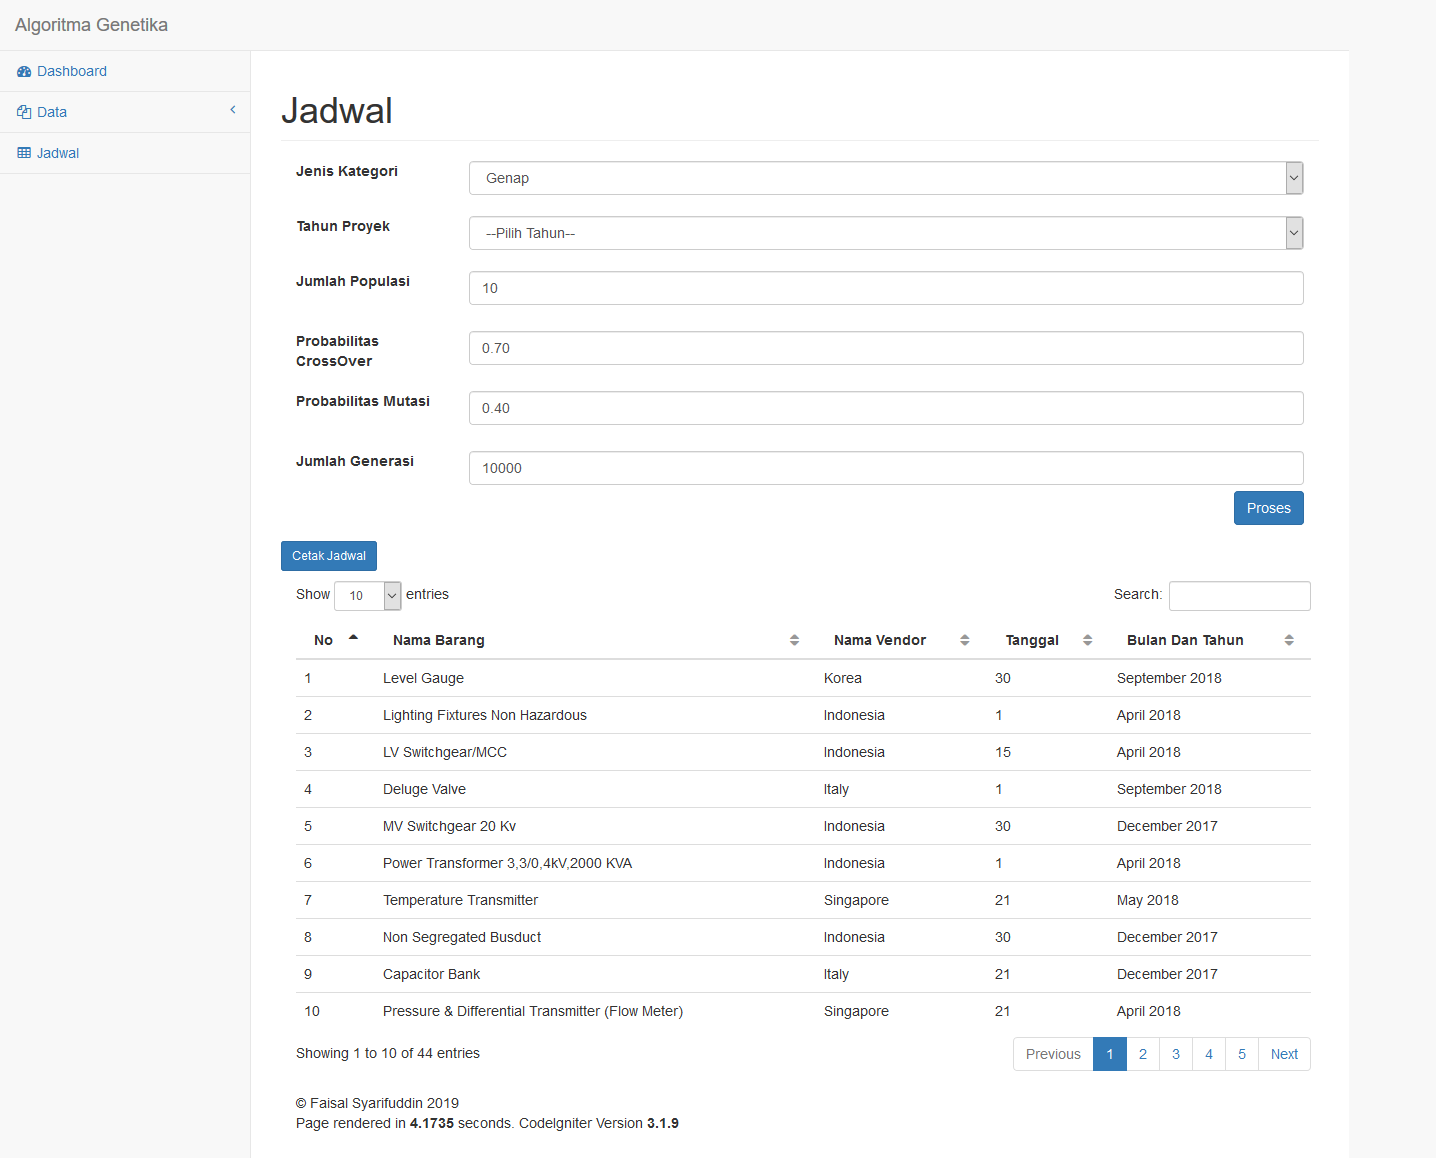
\includegraphics[width=0.6\textwidth]{figures/GA15.png}
        		\label{GA15}
    		\end{figure}
        \end{enumerate}
\end{enumerate}